\section{System analysis}
\phantomsection

\subsection{Motivation and the problem description}

\subsection{Existing solutions and their drawbacks}

\subsection {Proposed solution}
To create a useful application, it is really important to know what the market needs. 

Kyno should be capable of:

\begin{itemize}
\item Helping getting read of injuries, promote muscular function and mobility, to work muscles and the area with injuries, strengthen the muscles and joints so that they perform better.
\item During the exercise the tools that will help on rehabilitation will be the users hands only(not other tools, weights)

\item The UI should be intiutive, easy to use, clean and not very complicated. The UX must be great with not so many pop ups, additional panels. The application should provide to the user at least 3 which are most used and most useful for injuries recovery.
\item Have a price accordingly to the local and external market. Current solutions that involves technologies are way way more expensive then what I proprose. Thus, the price range must be affordable for the local and external market.
 
\end{itemize}
- 



\subsection{What problem is being solved}

All the program above does, when executed, is display "hello, world!" on the user's screen. You might have guessed as much just by looking over the code—and ignoring anything that didn't make sense! But what's with all the curly braces ({ and })? What's System.out? What does class Hello mean? And public static void main(String [] args)? Let's not even go there. 

Suffice it to say that, when it comes to learning to program, there's quite a learning curve with languages like Java. Before you can begin to solve problems, you must first learn to read and write a new language, even if the task at hand is relatively simple (e.g., "hello, world!"). And whereas you might still understand a foreigner who mispronounces some English word, computers aren't so forgiving when it comes to mistakes. Leave out a semicolon, and the program above won't even work! 

Learning to program is ultimately about learning to think logically and to approach problems methodically. The building blocks out of which a programmer constructs solutions, meanwhile, are relatively simple. Common in programming, for instance, are "loops" (whereby a program does something multiple times) and "conditions" (whereby a program only does something under certain circumstances. Also common are "variables" (so that a program, like a mathematician, can remember certain values). 

For many students, the seemingly cryptic syntax of languages like Java tends to get in the way of mastery of such relatively simple constructs as these. There we turn our attention to the application I developed before we tackle a language like Java, a "new programming language" that lets you create your own animations and interactive art. This desktop application is just as useful (and fun) for budding computer scientists. By representing programs' building blocks with color-coded blocks (cubes and other 3d polygons), this desktop application "lowers the bar" to programming, allowing budding computer scientists to focus on problems rather than syntax, to master programmatic constructs rather than syntax. But, for now, we focus on programming itself. It just so happens that programming, for now, will be more like putting together a 3d puzzle construction in VR than writing Greek. 

\subsection{Why this problem is important}

The term ‘UX ’ is used to refer to the approaches and methods employed to make sure that an application is entirely tailored and customized for its target market. If a platform does not appeal to a certain type of audience, it is likely to be quickly forgotten. That's why there should be a change in the way we are programming. The UX of my application will bring to the user changes in understanding the concept of programming and the world we live in by encouraging him to develope the following skills.

\begin{itemize}
\item{Information Skill}

"By programming in this desktop application, users learn to select, create and manage different forms of media, animation and arts. This way they become more critical into analyzing the world they created around them."
\item{Communication Skills}

"Nowdays it's not all about just the ability to read and write text (code). This VR enages users in choosing, interacting with a large variety of media to express their creativity.
 
\item{Critical and System Thinking}

"As they learn and interact with the programmable blocks, user become commited in critical and system thinking. During process of creation, users need to coordinate the timing and interaction between the programmable moving objects and themselves."

\item{Creativity Curiosity}

"It encourages amazing creative thinking, an  increasing skill in today's exponantially chaning world, in seeking different solutions to unexpected problems, not just learning how to solve a well given problem, but being always prepared to come up with new ideas, new solutions as new challengies occur."

\item{Interpersonal Skills}

"Because of the ability to program and literally interact through VR hands with programmable blocks, the "programming code" is more readable then other programming languages."

\end{itemize}

\subsection{Other products on the market}

Scratch \cite{sk} is an online program that kids as young as 5 years can use to express their online creations artistically while collaborating and sharing with other online users. Scratch has an intuitive drag-and-drop interface as shown in figure \ref{figI1} where the users will choose blocks of instructions to perform tasks.

Scratch is the work of MIT media lab and has a large number of Users creating and sharing their Projects online. Scratch is highly touted as the next generation tool to help kids prepare for the 21st century.

Various types of Projects can be created using Scratch like Stories, Animations, Games and even interaction with the Physical World

By creating projects in Scratch, kids will learn to think about designing stuff before building, will learn to solve problems creatively, express the ideas that are close to them and work collaboratively with others. Kids will also learn to share their work, present their work to others and get feedback and also comment on others projects. These are some of the most important skill sets needed for the 21st Century.
We turn our attention first to statements. 

\begin{figure}[!ht]
\renewcommand\thefigure{I.1} % Make this Figure I.1
\centering
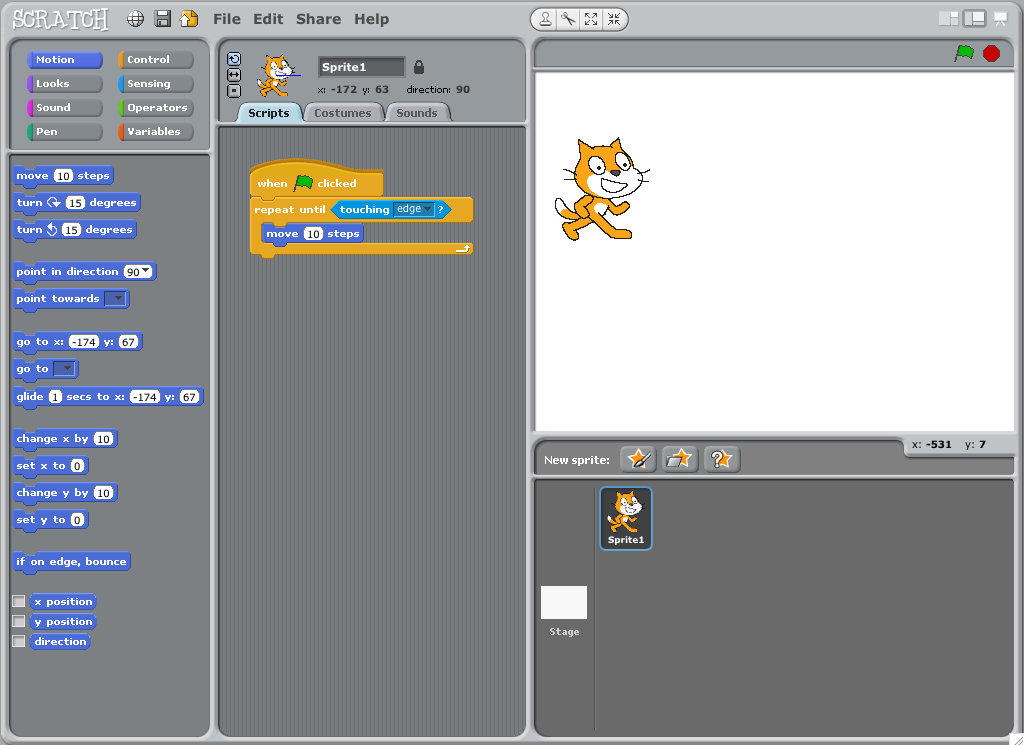
\includegraphics[width=10cm]{scratch.png}
\caption{The Scratch user interface }\label{figI1}
\end{figure}

\subsubsection{Advantages}

This are some of the advatages of Scratch while a explored it.

\begin{itemize}
\item Simple to use.
\item Suitable for children of all ages.
\item Most if not all of the coding is done for you, so all you have to worry about is how to put blocks \item together.
\item Cros-Curricular.
\item Friendly user interface.
\end{itemize}


\subsubsection{Disadvantages}
This are some of the disadvantages of Scratch while a explored it.
\begin{itemize}

\item Hard to use at first.
\item Simple sprites and graphics (you cannot use your own graphics).
\item If there is a bug in the engine, unless it is open source you can't fix it.
\item It's sprite based (only 2D)
\item Not suitable experienced programmers
	 
\end{itemize}



\subsection{Short thesis description}
Entering the application, the user will be in a wide room where he will be provided with a menu of programmable 3d objects such as cubes and other 3d primitives. With the help of Leap Motion he will be able to take those objects and to create blocks where after a push of a button the object that was programmed will behave accordingly to the block definition that user created previously. The programmable objects will have functionalities such as variables, methods, loops, structures. The user will enhance his VR experience even more by wearing Oculus Rift. It is going to be written in C-sharp programming language using Unity Game Engine. Also for this I will need Oculus Rift SDK for VR and Leap Motion SDK for virtual hands. The first prototype should be able to do handle minimal functionality from the system like rotating an object, moving it.

How will this blocks be created? Through sticking different 3d objects together (like tetris game).

\subsection{Chapters description}
	\begin{itemize}
	\item System Analysis
	\\
	This approach breaks systems analysis into 5 \cite{sa} phases:\\
	Scope Definition: denoting an instrument for observing, viewing, or examining\\
	Problem analysis: analyzing the problem that arises\\
	Requirements analysis: determining the conditions that need to be met\\
	Logical design: looking at the logical relationship among the objects\\
	Decision analysis: making a final decision
	
	\item {Implementation and Used Technologies}
	\item {Architecture of the System}
	\item {Economic Analysis}
	\end{itemize}
\clearpage
\clearpage